\section{Resultados}

\newread\tmp

\openin\tmp=../exp/shopping.s.entropy
\read\tmp to \ShoppingSEntropy
\closein\tmp

\openin\tmp=../exp/shopping.s1.entropy
\read\tmp to \ShoppingSOneEntropy
\closein\tmp

\openin\tmp=../exp/starbucks.s.entropy
\read\tmp to \StarbucksSEntropy
\closein\tmp

\openin\tmp=../exp/starbucks.s1.entropy
\read\tmp to \StarbucksSOneEntropy
\closein\tmp

\openin\tmp=../exp/wired_lan.s.entropy
\read\tmp to \WiredLanSEntropy
\closein\tmp

\openin\tmp=../exp/wired_lan.s1.entropy
\read\tmp to \WiredLanSOneEntropy
\closein\tmp

\subsection{Escenario 1 (Red cableada)}

\begin{tikzpicture}[baseline]
    \begin{axis}[
            title={},
            xlabel={Símbolo (Destino)},
            ylabel={Cantidad de información},
            scaled x ticks=false,
            scaled y ticks=false,
            width=0.45\textwidth,
            height=0.35\textwidth,
            bar width=2cm,
            ymin=0,
            enlarge x limits=0.65,
            xtick=data,
            major tick length=0,
            xticklabels={$s_{\texttt{UNICAST}}$, $s_{\texttt{BROADCAST}}$},
            x tick label style={rotate=80,anchor=east,font=\small},
            legend entries={$H(\mathcal{S})$,$H_{\max}(\mathcal{S})$},
            legend style={
                legend cell align=left,
                legend pos=north east
            }
        ]
        \addplot[
                ybar,
                fill=blue!10,
                draw=blue,
                forget plot
            ] table[x=IsBroadcast,y=Information]{../exp/wired_lan.s.information};
        \addplot[mark=none, blue, thick, update limits=false] {\WiredLanSEntropy};
        \addplot[mark=none, blue, thick, dashed, update limits=false] {1};
    \end{axis}
\end{tikzpicture}

\begin{tikzpicture}[baseline]
    \begin{axis}[
            title={},
            xlabel={Símbolo (Dirección IP)},
            ylabel={Cantidad de información},
            scaled x ticks=false,
            scaled y ticks=false,
            width=0.45\textwidth,
            height=0.35\textwidth,
            legend pos=outer north east,
            legend cell align=left,
            ymin=0,
            xtick=data,
            xticklabels from table={../exp/wired_lan.s1.information}{IP},
            x tick label style={rotate=80,anchor=east,font=\small}
        ]
        \addplot [
                ybar,
                fill=blue!10,
                draw=blue,
                select coords between index={0}{20}
            ] table[x=X-Pos,y=Information]{../exp/wired_lan.s1.information};

        \coordinate (A) at (axis cs:0,\WiredLanSOneEntropy);
        \coordinate (O1) at (rel axis cs:0,0);
        \coordinate (O2) at (rel axis cs:1,0);

        \draw [blue, thick] (A -| O1) -- (A -| O2);

    \end{axis}
\end{tikzpicture}

\begin{figure}[H]
    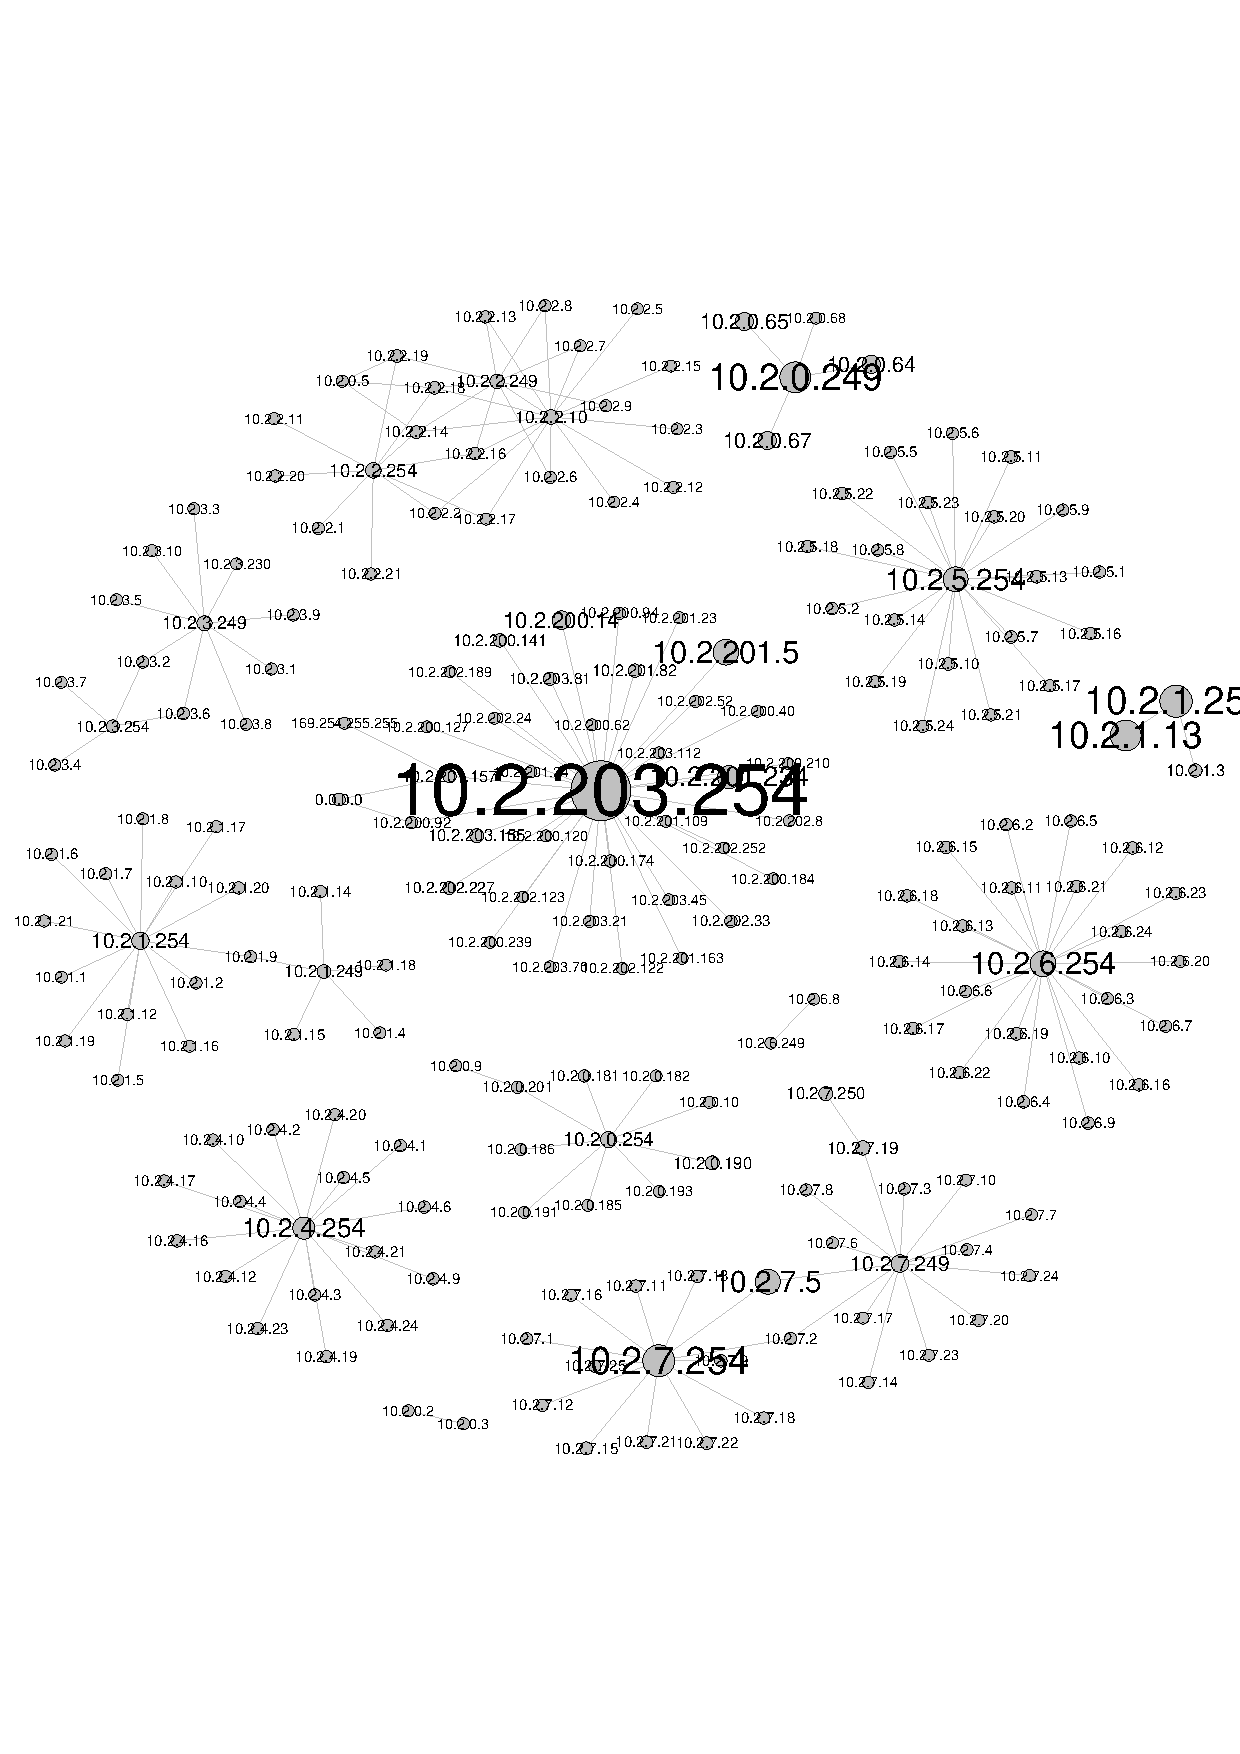
\includegraphics[scale=0.4]{figures/wired_lan.pdf}
    \caption{Red de mensajes \texttt{ARP} para captura de red cableada.}
\end{figure}

\subsection{Escenario 2 (\emph{Shopping})}

La principal motivación para estudiar esta red fue poder observar un medio con
mucha actividad, el hecho de que se tratara de una red inalámbrica permitió además
contrastar las diferencias frente a la primer captura sobre una red cableada.

Primero se analizarán los resultados obtenidos para la fuente $\mathcal{S}$.

\begin{figure}[h]
	\figdef[dim]{figures/shopping_s_fig}
	\caption{Cantidad de información por símbolo y entropía de $\mathcal{S}$.}
    \label{res:esc2:fig1}
\end{figure}

Como es posible observar en la Figura \ref{res:esc2:fig1} la entropía de
$\mathcal{S}$ no es máxima. La misma posee un valor relativamente inferior lo
cual indica que la fuente es bastante predecible. Se puede apreciar cómo la
cantidad de información que aporta $s_{\texttt{UNICAST}}$ es mínima con respecto
a $s_{\texttt{BROADCAST}}$. Esto se debe al bajo número de paquetes con destino
broadcast en la red.

Una posible hipótesis a este resultado es el hecho de que se trate de la red
inalámbrica de un centro comercial. Es razonable asumir que los hosts conectados
a la misma más que comunicarse entre ellos estarán accediendo mediante el
gateway a Internet.

Para ello, los mismos necesitan la dirección física asociada a la dirección
\texttt{IP} del gateway. Aquí es donde entra en juego \texttt{ARP}, donde los
hosts a través de mensajes broadcast \texttt{WHO-HAS} consultan por ella. Cuando
este mensaje llega al default gateway además de responder con su dirección
física a cada host que consultó por él, el dispositivo guarda la asociación
entre la dirección \texttt{IP} que originó el mensaje junto a su dirección física.

De esta manera, en un principio los únicos mensajes broadcast presentes son los
que resultan de los paquetes \texttt{ARP} generados por los hosts con el fin de
tener la dirección física del gateway. Una vez hecho esto, el gateway ya conoce
a los hosts por lo tanto cualquier comunicación entre ambos resulta en un
intercambio de paquetes unicast.

Habiendo dicho esto, asumiendo que la hipótesis es cierta, sería correcto
afirmar que existe una relación entre los protocolos de control como
\texttt{ARP} y la fuente $\mathcal{S}$. Si hubiera habido comunicación entre los
nodos de la red entonces el número de broadcasts habría sido necesariamente
mayor dado que en lugar de sólo consultar por la dirección física del gateway
también se lo habría hecho por el resto de los hosts.

A continuación se analizarán los resultados obtenidos para la fuente
$\mathcal{S}_1$.

\begin{figure}[h]
	\figdef[dim]{figures/shopping_s1_fig}
	\caption{Cantidad de información por símbolo y entropía de $\mathcal{S}_1$.}
    \label{res:esc2:fig2}
\end{figure}

Estudiando el tráfico \texttt{ARP} de la captura de esta red se notaron algunas
características que merecen ser mencionadas. La primera es que corroborando la
hipótesis sugerida en el análisis anterior, los mensajes del tipo
\texttt{WHO-HAS} iban todos dirigidos al gateway de la red. La segunda,
fuertemente relacionada con la primera, es el hecho de que el gateway es el
único generando respuestas \texttt{IS-AT} a los hosts y prácticamente no realiza
ningún pedido \texttt{WHO-HAS}.

Ambos comportamientos pueden ser justificados con la hipótesis sobre el tipo de
comunicaciones que se establecen en una red inalámbrica dentro de un centro
comercial. Además, buscando información sobre los routers inalámbricos
utilizados para este tipo de instalaciones se encontró que el \emph{timeout} de
las tablas \texttt{ARP} puede llegar a valores de hasta 4 horas. Esto tiene
sentido puesto que estos dispositivos tienen la capacidad de almacenamiento
necesaria para no tener que preocuparse por quedarse sin espacio para las
entradas.

El modelo utilizado para la fuente $\mathcal{S}_1$ dio un total de 30 nodos en la
red. En la Figura \ref{res:esc2:fig2} se muestran los primeros 20 ordenados por
la cantidad de información que brindan, donde se puede apreciar como hay un
único dispositivo cuyo nivel de información está por debajo del de la entropía
calculada.

Este nodo distinguido resulta ser el gateway de la red estudiada. Su bajo aporte
de información tiene sentido puesto que con el modelo utilizado por cada mensaje
\texttt{WHO-HAS} que lo tenga como destino u origen aumenta la probabilidad de
ocurrencia de su símbolo. Por todo lo discutido anteriormente esto
necesariamente lo vuelve el símbolo con mayor probabilidad de aparición y como
consecuencia el que menor información aporta.

Por último, en la Figura \ref{res:esc2:fig3} se tiene la visualización del
tráfico \texttt{ARP} donde el tamaño de los nodos es proporcional a la
probabilidad de sus símbolos en la fuente $\mathcal{S}_1$. Aquí queda más que
evidente el rol de gateway del nodo distinguido, donde todo el tráfico del
protocolo es entre los hosts y el mismo.

Con respecto a la posibilidad de utilizar esta fuente como método para encontrar
los default gateways, como en este caso resultó efectivo uno podría verse
tentado a decir que el mismo es efectivo en la tarea. Sin embargo, existen muchos
factores que podrían llegar a alterar los resultados obtenidos generando
conclusiones incongruentes. Por ejemplo, la captura sobre la cual se realizó
todo este estudio fue hecha en un punto donde llegaba la señal de un único
\emph{access point}. Si hubieran habido más de estos, dependiendo dónde se
realizaba físicamente la captura se habrían obtenido más o menos paquetes
dirigidos a los mismos. Por lo tanto podría haber ocurrido que habiendo dos
default gateways por el simple hecho de que no llegaran a capturarse suficientes
paquetes dirigidos a uno de ellos el símbolo representando al mismo tuviera una
probabilidad asociada muy baja generando entonces mucha información en la fuente
$\mathcal{S}_1$ quedando por encima de la entropía calculada.

\begin{figure}[h!]
	\figdef[dim]{figures/shopping_arp_fig}
    \caption{Red de mensajes \texttt{ARP} para captura del shopping.}
    \label{res:esc2:fig3}
\end{figure}

\vfill % used to avoid funny stretching between paragraphs

\subsection{Escenario 3 (\emph{Starbucks})}

\begin{tikzpicture}[baseline]
    \begin{axis}[
            title={},
            xlabel={Símbolo (Destino)},
            ylabel={Cantidad de información},
            scaled x ticks=false,
            scaled y ticks=false,
            width=0.45\textwidth,
            height=0.35\textwidth,
            bar width=2cm,
            ymin=0,
            enlarge x limits=0.65,
            xtick=data,
            major tick length=0,
            xticklabels={$s_{\texttt{UNICAST}}$, $s_{\texttt{BROADCAST}}$},
            x tick label style={rotate=80,anchor=east,font=\small},
            legend entries={$H(\mathcal{S})$,$H_{\max}(\mathcal{S})$},
            legend style={
                legend cell align=left,
                legend pos=north west
            }
        ]
        \addplot[
                ybar,
                fill=blue!10,
                draw=blue,
                forget plot
            ] table[x=IsBroadcast,y=Information]{../exp/starbucks.s.information};
        \addplot[mark=none, blue, thick, update limits=false] {\StarbucksSEntropy};
        \addplot[mark=none, blue, thick, dashed, update limits=false] {1};
    \end{axis}
\end{tikzpicture}

\begin{tikzpicture}[baseline]
    \begin{axis}[
            title={},
            xlabel={Símbolo (Dirección IP)},
            ylabel={Cantidad de información},
            scaled x ticks=false,
            scaled y ticks=false,
            width=0.45\textwidth,
            height=0.35\textwidth,
            legend pos=outer north east,
            legend cell align=left,
            ymin=0,
            xtick=data,
            xticklabels from table={../exp/starbucks.s1.information}{IP},
            x tick label style={rotate=80,anchor=east,font=\small}
        ]
        \addplot [ybar, fill=blue!10, draw=blue] table[x=X-Pos,y=Information]
                {../exp/starbucks.s1.information};

        \coordinate (A) at (axis cs:0,\StarbucksSOneEntropy);
        \coordinate (O1) at (rel axis cs:0,0);
        \coordinate (O2) at (rel axis cs:1,0);

        \draw [blue, thick] (A -| O1) -- (A -| O2);

    \end{axis}
\end{tikzpicture}

\begin{figure}[H]
    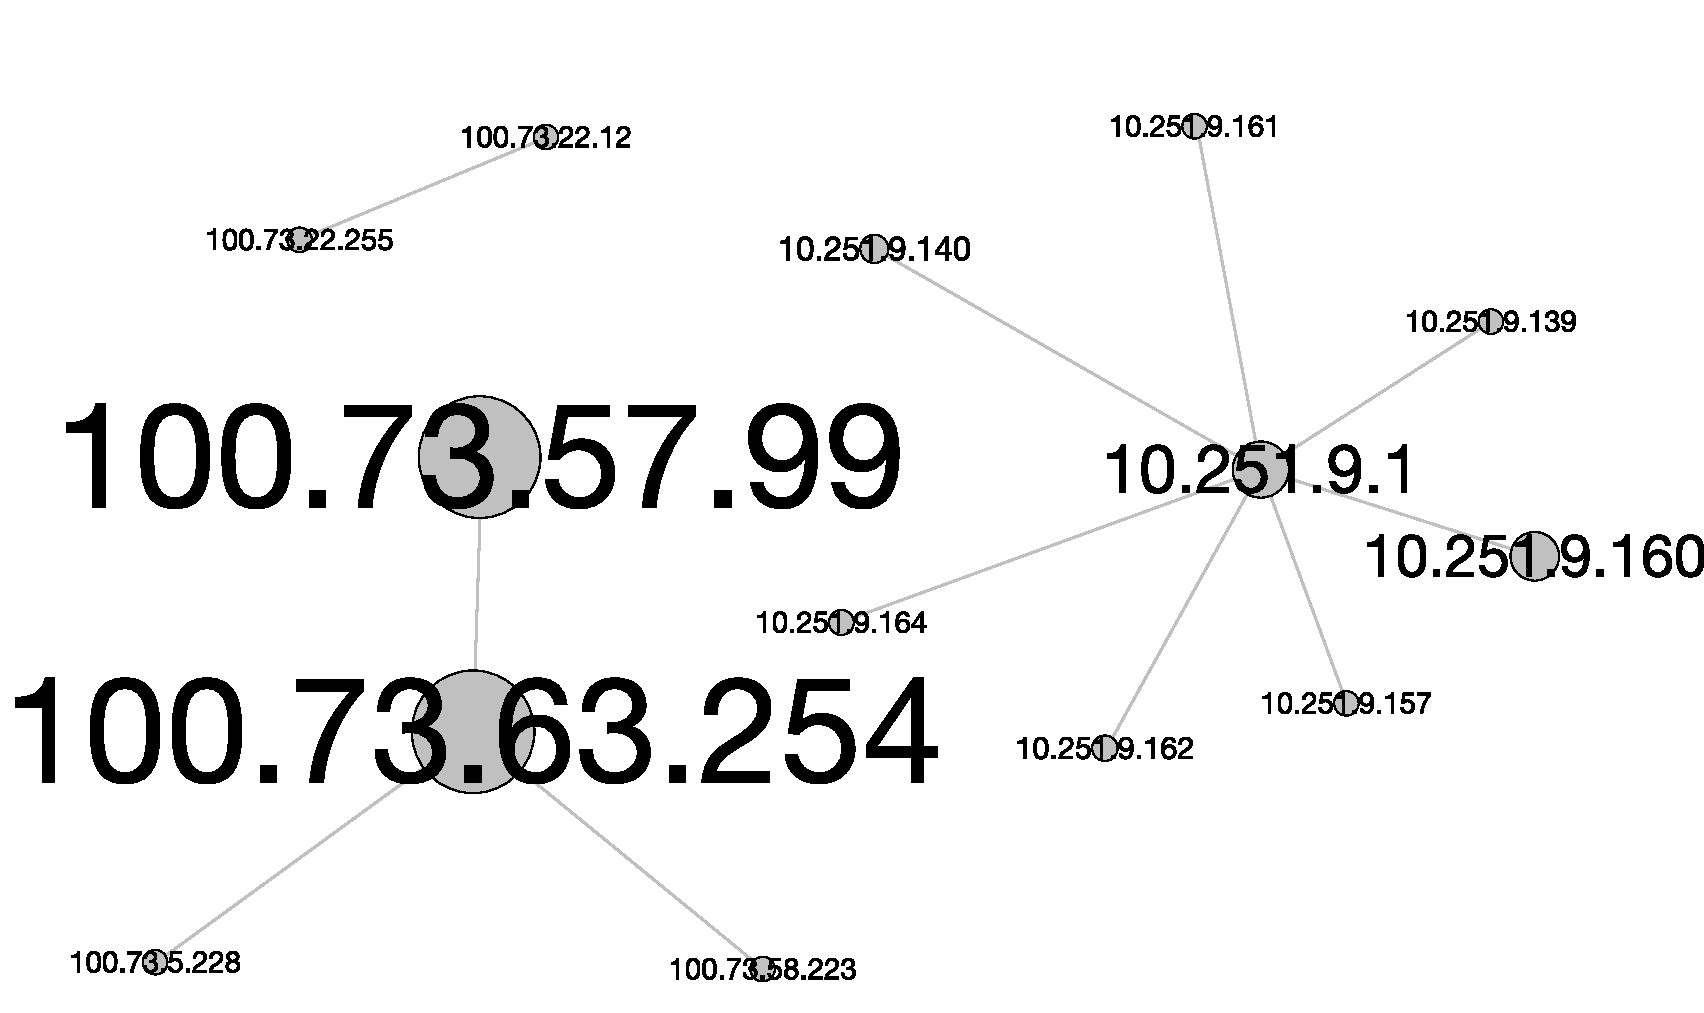
\includegraphics[scale=0.4]{figures/starbucks.pdf}
    \caption{Red de mensajes \texttt{ARP} para captura del Starbucks.}
\end{figure}
